\documentclass[t]{beamer}
\usepackage{beamerthemesplit}
\usepackage{xcolor}
\usepackage{color}
\usetheme{USC}
\begin{document}

\graphicspath{ {../Manuscript/figures/}{Graphics/} }

\title[USC Viterbi School of Engineering]{Probabilistic estimation of link travel times in dynamic road networks}  
\author[Mohammad Asghari]{Mohammad Asghari\\ \small{masghari@usc.edu}\\ \vspace{0.1in} \tiny{Joint work with Tobias Emrich, Ugur Demiryurek and Cyrus Shahabi}}

\date{Nov 6, 2015} 

\begin{frame}
\titlepage
\begin{columns}
  \column{.2\textwidth}
  \begin{center}
    
\includegraphics[height=1.5cm]{viterbi_logo.jpg}   
  \end{center}
  \column{.6\textwidth}
  \column{.2\textwidth}
  \begin{center}
    
\includegraphics[height=1.5cm]{imsc_logo.jpg}   
  \end{center}
\end{columns} 
\end{frame}

\begin{frame}\frametitle{Outline}\tableofcontents
\end{frame} 

\section{Introduction}
\begin{frame}\frametitle{Motivation}
\vspace{-0.2in}
\only<1-2>{
\begin{columns}
	\column{0.5\textwidth}
		\begin{center}
			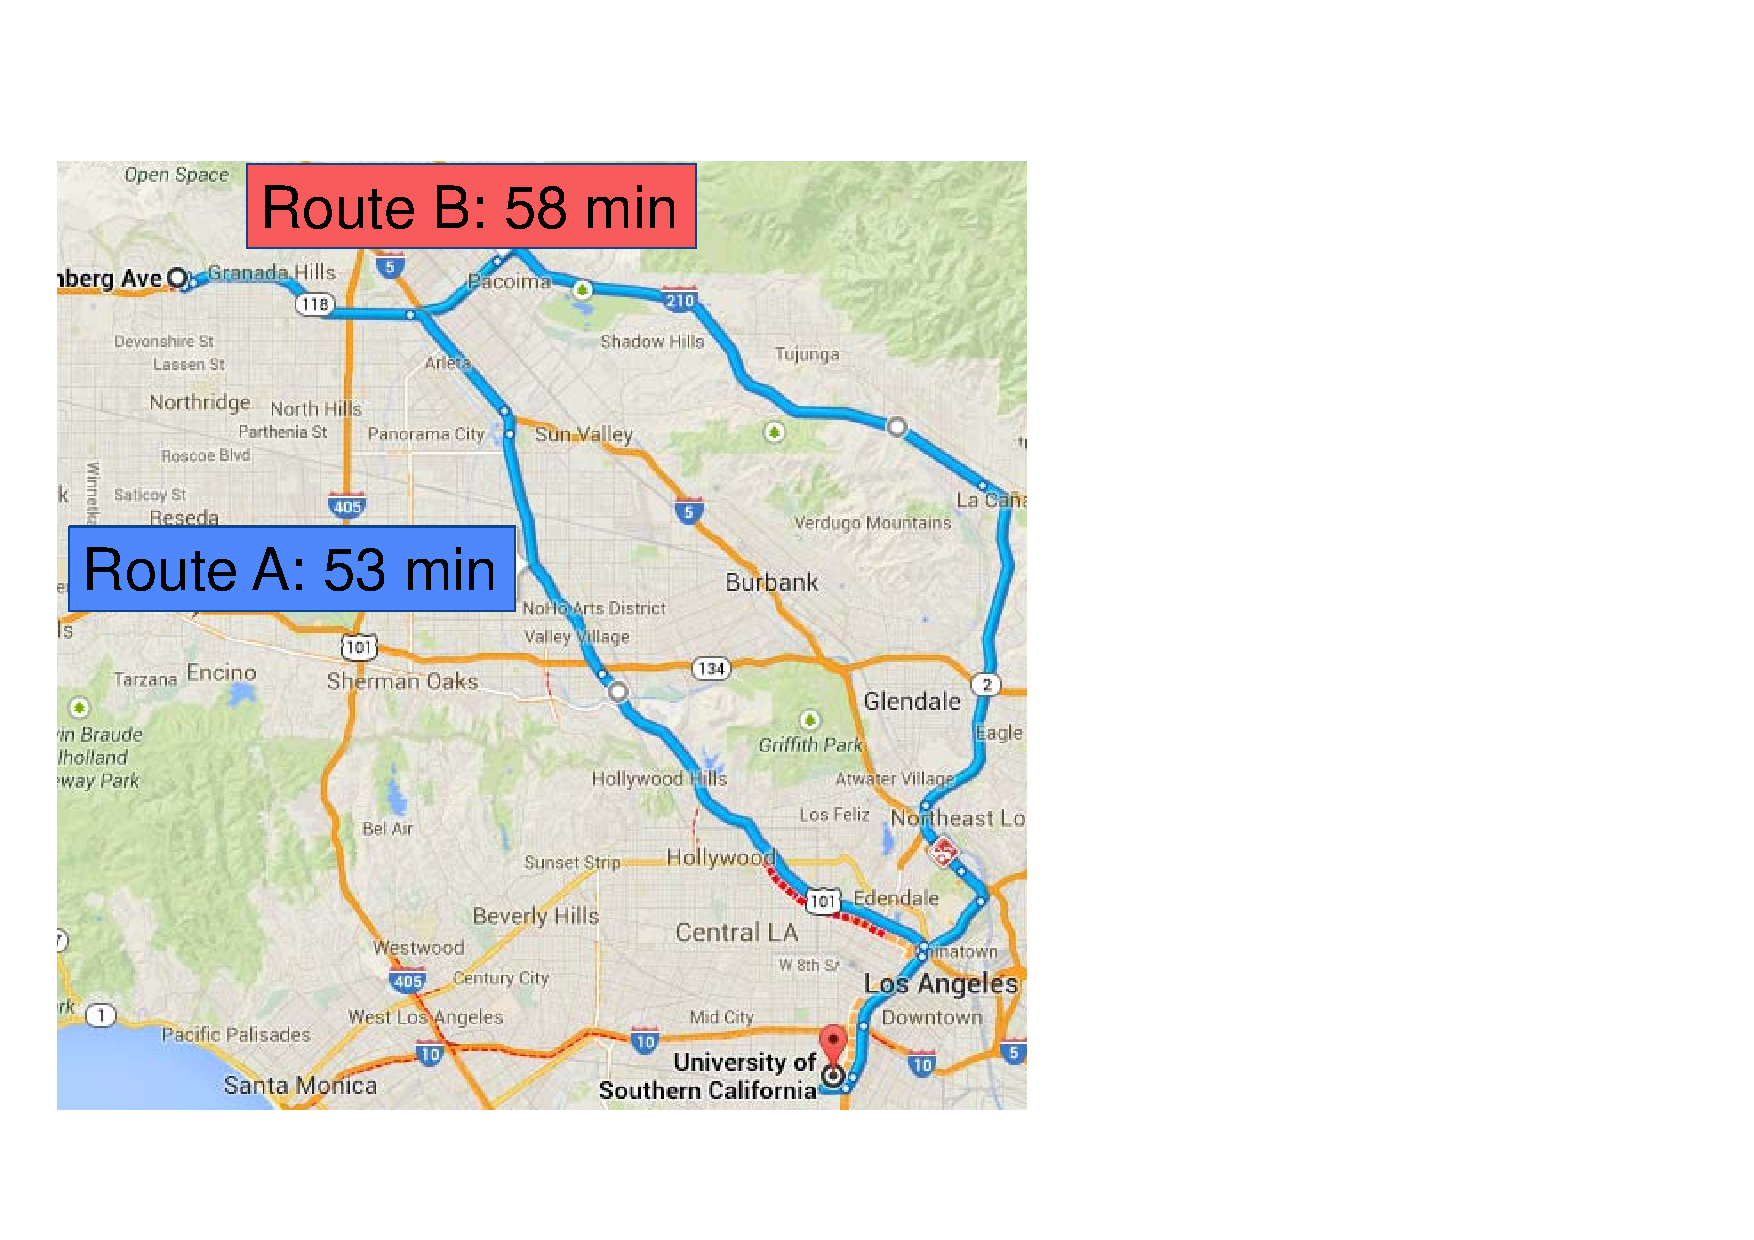
\includegraphics[scale=0.25]{motivation1.pdf}
		\end{center}
	\column{0.5\textwidth}
\end{columns}
}
\only<3->{
\begin{columns}
	\column{0.5\textwidth}
		\begin{center}
			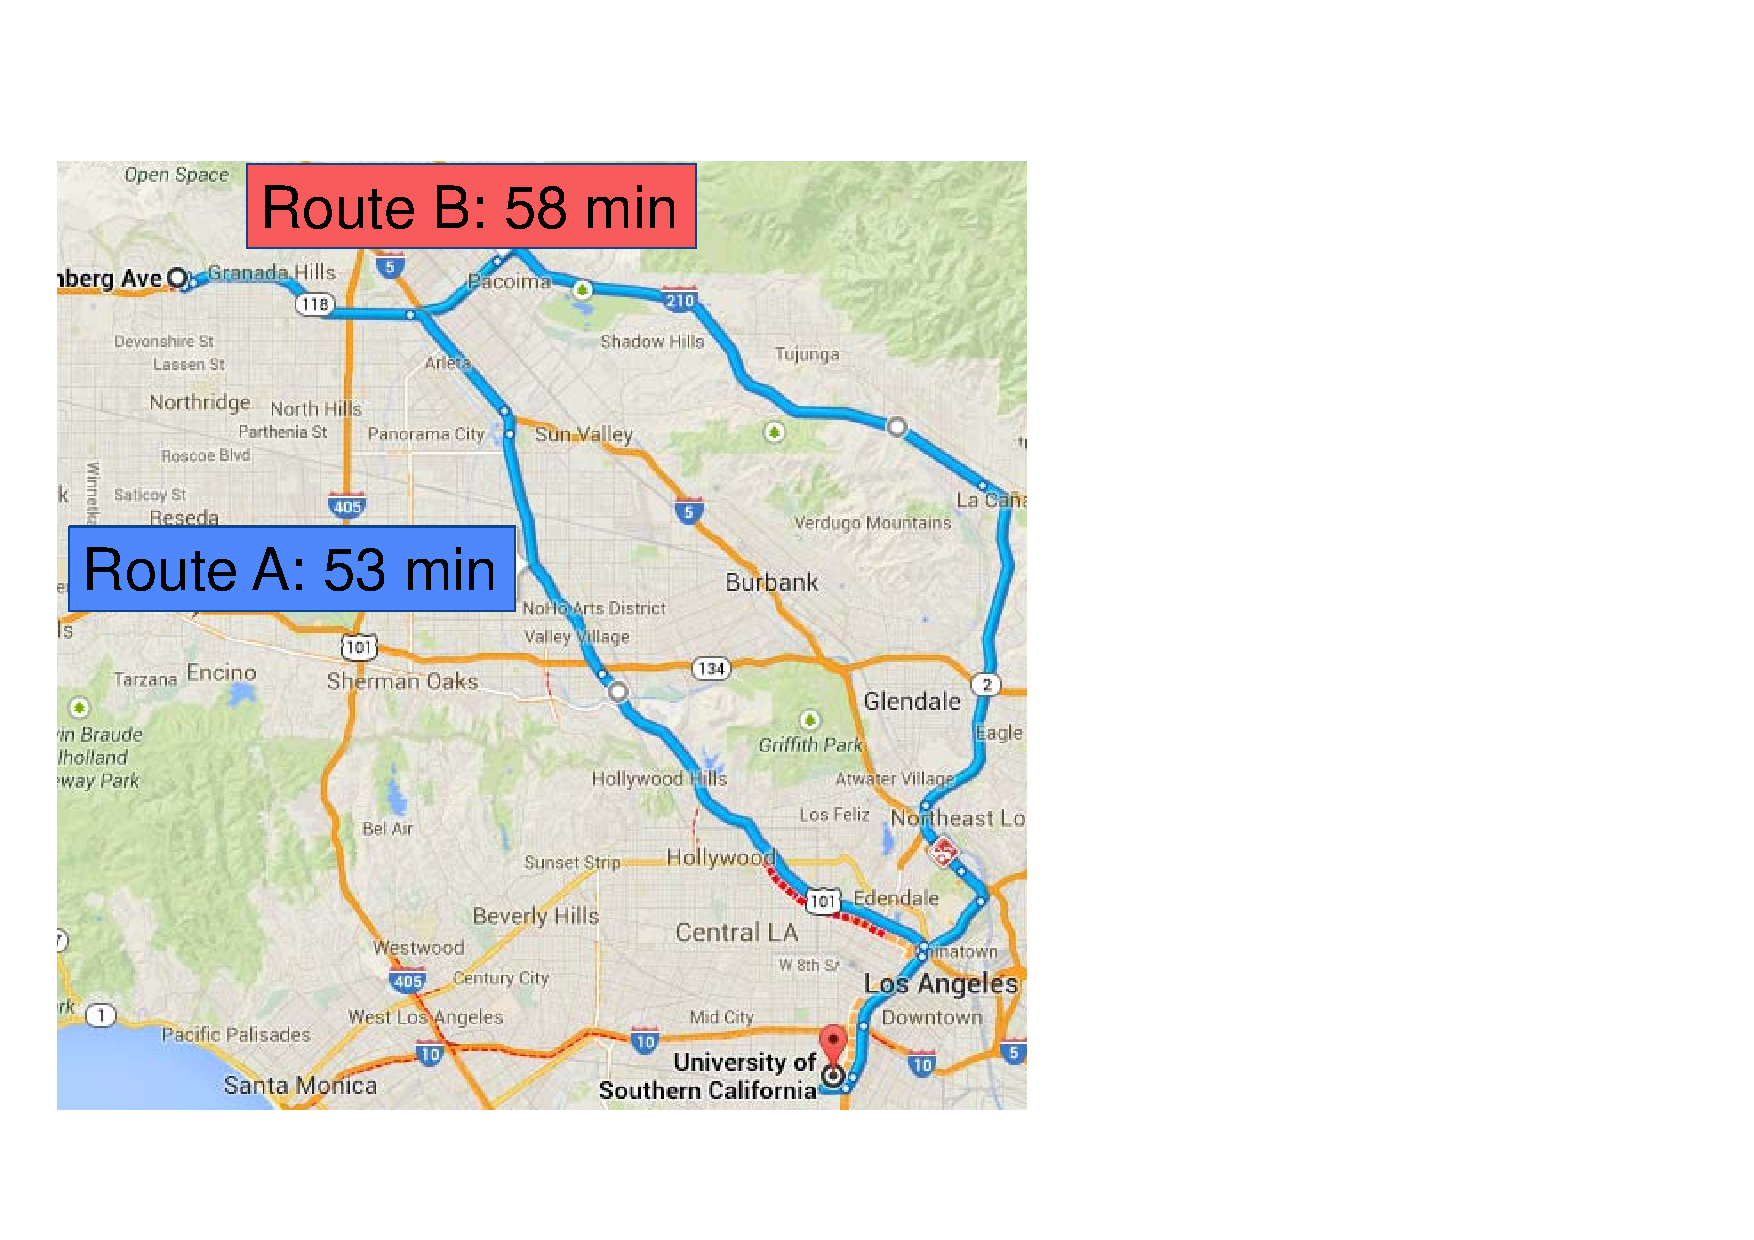
\includegraphics[scale=0.25]{motivation1.pdf}
		\end{center}
	\column{0.5\textwidth}
		\begin{center}
			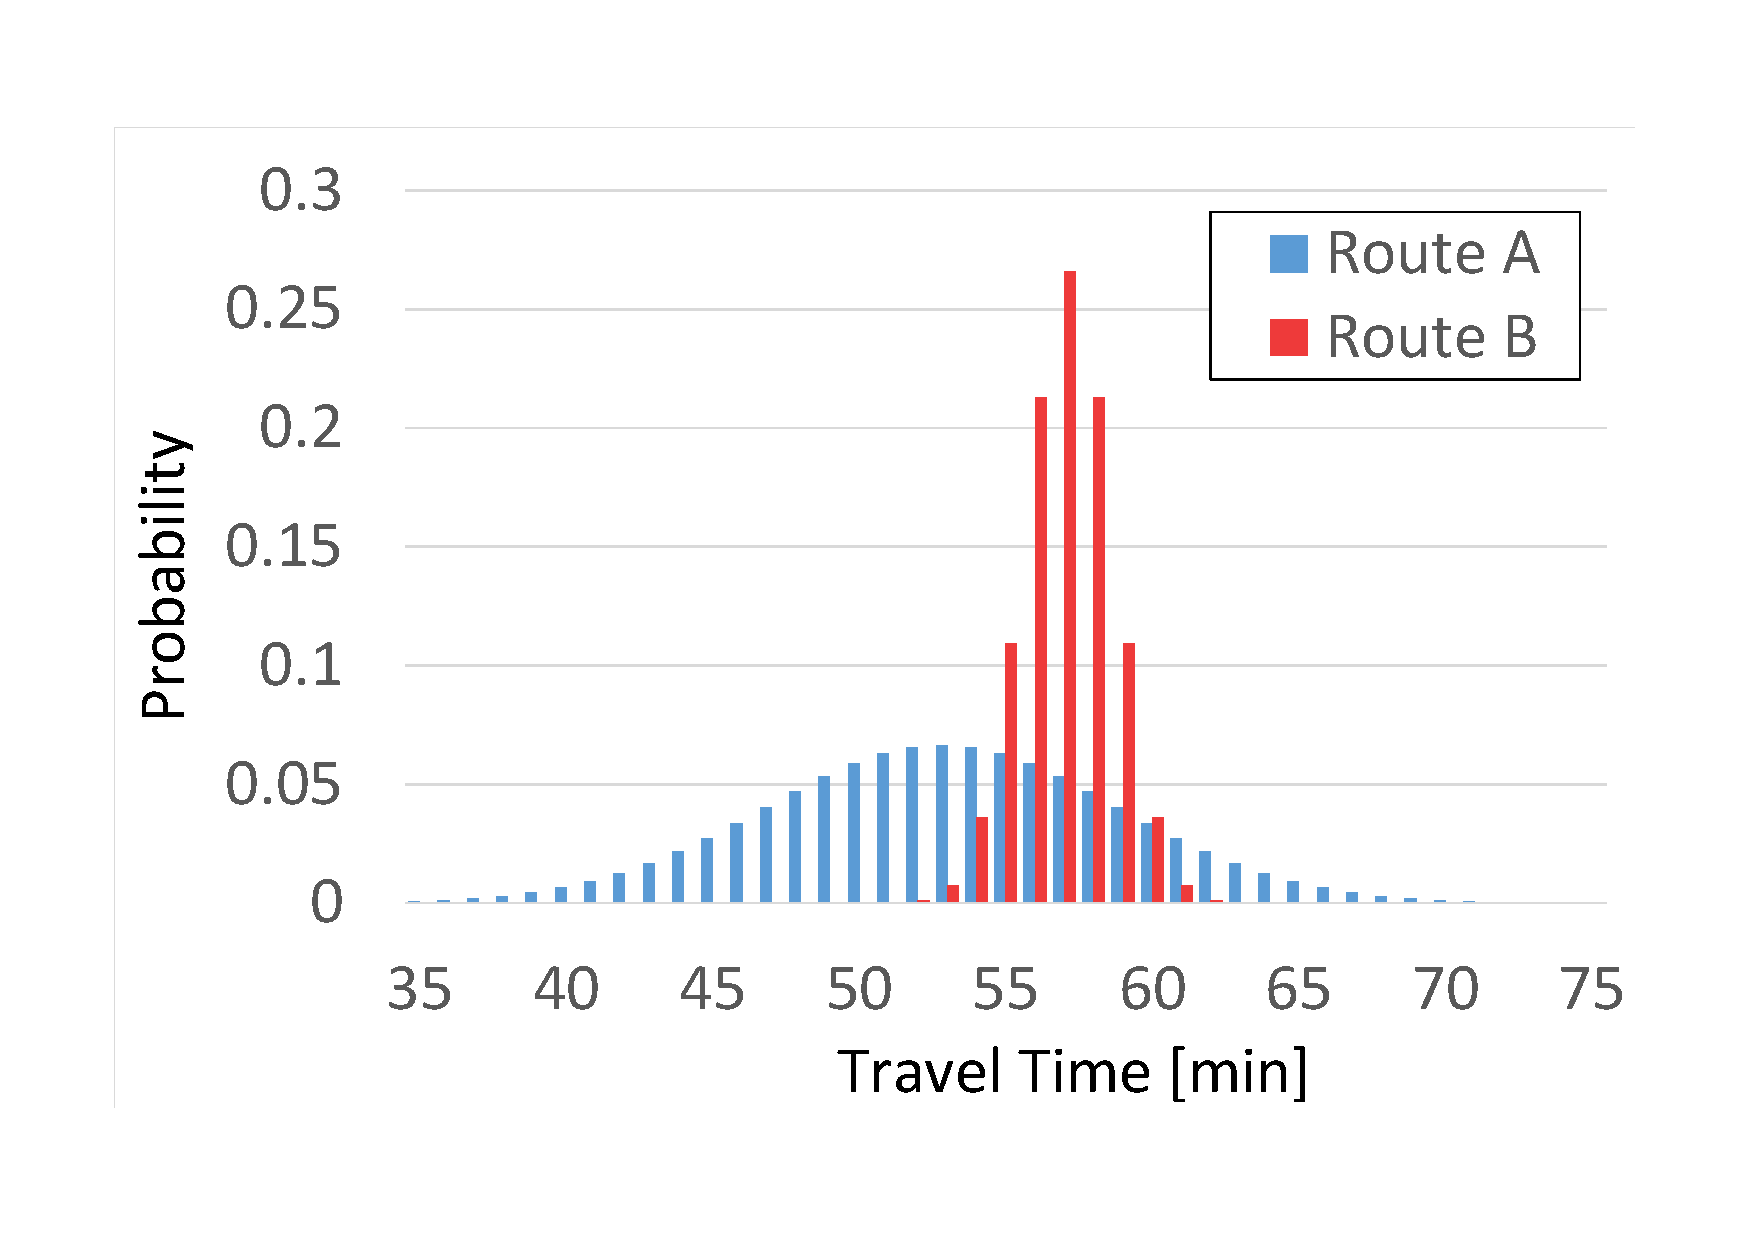
\includegraphics[scale=0.2]{motivation2.pdf}
		\end{center}
\end{columns}
}
\only<2->{
\begin{exampleblock}{}\textit{What's the probability of reaching campus in \textbf{at most} 60 minutes?}
\end{exampleblock}
}
\only<4>{
\begin{equation*}
\sum_{i \leq 60} P(i)
\end{equation*}
}
\only<5>{
\begin{itemize}
	\item \textcolor{blue}{Route A:} 89\%
	\item \textcolor{red}{Route B:} 99.2\%	
\end{itemize}
}
\end{frame}

\begin{frame}\frametitle{Probabilistic Travel Times}
\begin{columns}
\column{0.5\textwidth}
\only<2->{
How to compute the travel time \textit{PMF} for an entire route?
}
\only<3->{
\begin{itemize}
\item \tiny{H. Frank, \textit{Shortest paths in probabilistic graphs.}}
\item \tiny{E.D. Miller-Hooks et al., \textit{Least expected time paths in stochastic, time-varying transportation networks.}}
\item \tiny{Y.M. Nie et al., \textit{Shortest path problem considering on-time arrival probability.}}
\item ... 
\end{itemize}
}
\column{0.5\textwidth}
\begin{center}
	\vspace{-0.35in}
	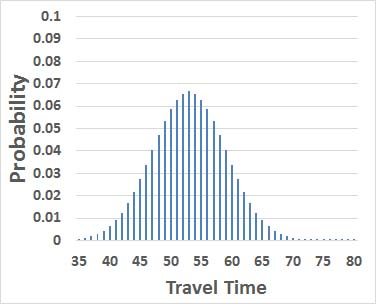
\includegraphics[scale=0.35]{Sample_PMF.jpg}
\end{center}
\end{columns}

\begin{columns}
\column{0.7\textwidth}
\only<4-5>{
\begin{center}
	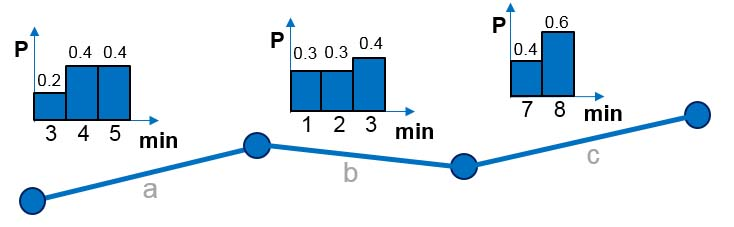
\includegraphics[scale=0.33]{route_construction1.jpg}
\end{center}
}
\only<6->{
\begin{center}
	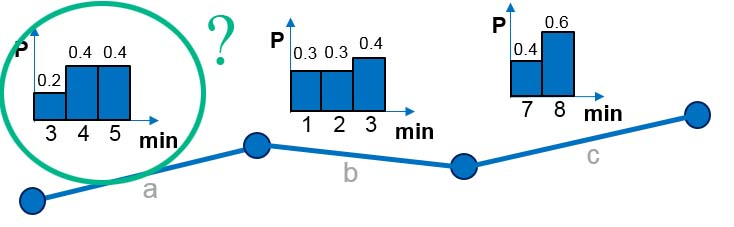
\includegraphics[scale=0.33]{route_construction2.jpg}
\end{center}
}
\column{0.3\textwidth}
\only<5->{
\begin{center}
	\vspace{0.2in}
	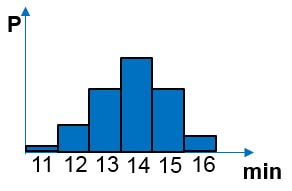
\includegraphics[scale=0.33]{sample_pmf2.jpg}
\end{center}
}
\end{columns}
\end{frame}

\section{Definitions}
\frame{\frametitle{Outline}\tableofcontents[currentsection]}

\begin{frame}\frametitle{Definitions}
\vspace{-0.2in}
\begin{block}{\textit{Probabilistic Link Travel Times \textit{(pltt)}}}
The probabilistic link travel time of link $(i,j)$, $c_{ij}^t(x)$, is the probability of taking $x$ seconds for a vehicle to traverse link $(i,j)$ starting at time $t$.
\end{block}
\only<2->{
\begin{alertblock}{Route PDF (\textbackslash PMF)}
If $p_{sd}$ is a path starting at $s$ and ending in $d$, $\pi_{sd}^t$ is the random variable representing the travel time on $p_{sd}$ when we start at time $t$. Accordingly, the route pdf, $J_{sd}^t(x)$, gives the probability of taking $x$ seconds for a vehicle to traverse $p_{sd}$ starting at time $t$
\end{alertblock}
}
\only<3>{
\begin{center}
	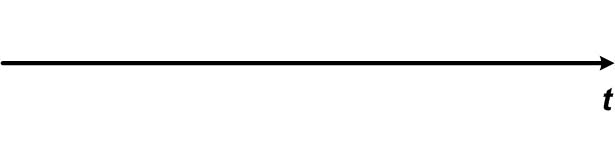
\includegraphics[scale=0.33]{times1.jpg}
\end{center}
}
\only<4>{
\begin{center}
	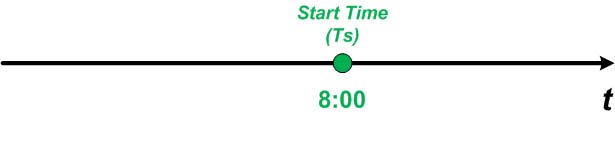
\includegraphics[scale=0.33]{times2.jpg}
\end{center}
}
\only<5>{
\begin{center}
	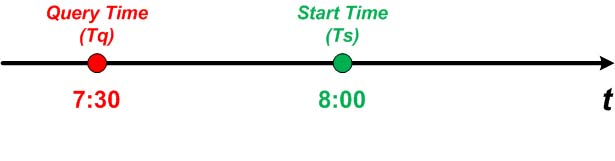
\includegraphics[scale=0.33]{times3.jpg}
\end{center}
}
\only<6>{
\begin{center}
	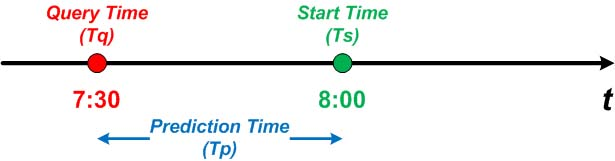
\includegraphics[scale=0.33]{times4.jpg}
\end{center}
}
\end{frame}

\section{Probabilistic Link Travel Times}
\frame{\frametitle{Outline}\tableofcontents[currentsection]}

\begin{frame}
\begin{itemize}
\item Historic Data Vs. Current Situation
\item<2-> PLTT Representation (Continuous Vs. Discrete)
\begin{itemize}
\item<3-> Continuous\\
\only<3>{
Link Travel times are normally or gamma distributed.
}
\only<4->{
Link Travel times are \textbf{normally} or gamma distributed
\begin{itemize}
\item $c_{ij}^t$ is characterized by a mean $\mu_{ij}^t$ and a standard deviation $\sigma_{ij}^t$.
\end{itemize}
}
\item<5-> Discrete\\

\only<6->{
We use b-discrete to discretize the time domain into intervals of length $\phi$:

\begin{equation*}
	T = \{ t | t = n \cdot \phi \wedge n \in \mathbb{N} \}
\end{equation*}
}

\only<7->{
Then the PMF $F_{ij}$ of link travel time $c_{ij}$ will be:
\begin{equation*}
	F_{ij}(b) = \begin{cases}\int_b^{b+\phi}f_{ij}(w)dw \qquad b =
	0,\phi,\ldots, (L-1)\phi\\
	\int_b^{\infty}f_{ij}(w)dw \qquad b =
	L \phi\\
	0 \qquad otherwise
	\end{cases} 
\end{equation*}
}
\end{itemize}
\end{itemize}
\end{frame}

\end{document}